\vzmstitle[\footnote{Работа выполнена при поддержке Российского фонда фундаментальных исследований (проект №~19-01-00244).}]{ОБ ОДНОЙ МОДЕЛИ НЕЛИНЕЙНОЙ СТОИМОСТИ ЛИКВИДНОСТИ ПРИ ДЕЛЬТА-ХЕДЖИРОВАНИИ ОПЦИОНОВ}
\vzmsauthor{Дышаев}{М.\,М.}
\vzmsinfo{Челябинск, Челябинский государственный университет; {\it Mikhail.Dyshaev@gmail.com}}
\vzmsauthor{Федоров}{В.\,Е.}
\vzmsinfo{Челябинск, Челябинский государственный университет; {\it kar@csu.ru}}
\vzmsauthor{Авилович}{А.\,С.}
\vzmsinfo{Челябинск, Челябинский государственный университет; {\it avilovich\_aas@bk.ru}}
\vzmscaption

Рассматривается модель Роджера и Сингха (2010) [1], позволяющая оценить нелинейную стоимость ликвидности базового актива при операциях дельта"=хеджирования в применении к рынку опционов на Московской Бирже.
В ней эффект недостаточной ликвидности проявляется как дополнительные затраты при операциях, которые, однако, не влияют на цену базового актива. Эти затраты отражают глубину книги ордеров. Влияние ликвидности, моделируемой таким образом, подобно влиянию транзакционных издержек, но в отличие от классических моделей имеет нелинейный характер и не пропорционально объёму сделок.

Пусть имеется средняя цена $S$ и книга лимитных ордеров (заявок на покупку и продажу, выставленных другими участниками), распределённая по обе стороны от средней цены $S$ с плотностью котировок $\rho(x)$, где $x$~--- относительная цена. Если трейдер приобретает $h$ единиц базового актива, он должен будет выкупить их через книгу ордеров до относительной цены $s$, определённой как
\begin{equation*}
h = \int\limits_1^s \rho(x)dx.
\end{equation*}
При этом он заплатит величину
\begin{equation*}
S=\int\limits_1^s x \rho(x) dx.
\end{equation*}
После совершения этой сделки средняя цена быстро возвращается к $S$, поэтому балансовая (так называемая <<бумажная>>) стоимость базового актива, который он только что купил, составляет $S \cdot h$. Следовательно, сравнивая фактическую и балансовую стоимость, трейдер имеет балансовый убыток, отражающий стоимость ликвидности, в сумме
\begin{equation*}
S l(h) = S \int\limits_1^s x \rho(x) dx - Sh = S \int\limits_1^s (x-1) \rho(x) dx.
\end{equation*}

В дальнейших исследованиях Роджер и Сингх использовали форму $l (h) = \frac12 \varepsilon h^2$, которая была выбрана из соображений управляемости уравнения Гамильтона~--- Якоби~--- Беллмана (см. Замечание и уравнение (3.12) в [1]). Для численных решений Роджер и Сингх приняли $\varepsilon = 0.00006$, основываясь на эмпирических заключениях о рынке акций.

Поскольку вид данной функции оказывает влияние на стоимость репликации портфеля опционов,  поставлена задача исследовать вид функции $l(h)$ для различных базовых активов, торгуемых на Московской Бирже. Были исследованы мгновенные состояния книги лимитных ордеров для фьючерса на курс доллар США~--- российский рубль Si-12.19 и для фьючерса BR-11.19 на нефть сорта Brent.

Результаты, представленные на рис.~1 показывают, что функция  $l(h)$, рассчитанная на основании рыночных данных, отличается от принятой в работе Роджера и Сингха. Множество точек, расположенных в правой части рисунка, соответствует книге ордеров для фьючерса на курс доллар США~--- российский рубль (синие точки). В средней части рисунка расположены значения функции $l(h)$, соответствующие книге ордеров для фьючерса на нефть сорта Brent (зелёные треугольники). Близко к оси ординат расположен график функции $l(h)$, соответствующий модели Роджера и Сингха (фиолетовые крестики).
\begin{figure}
	\centering
	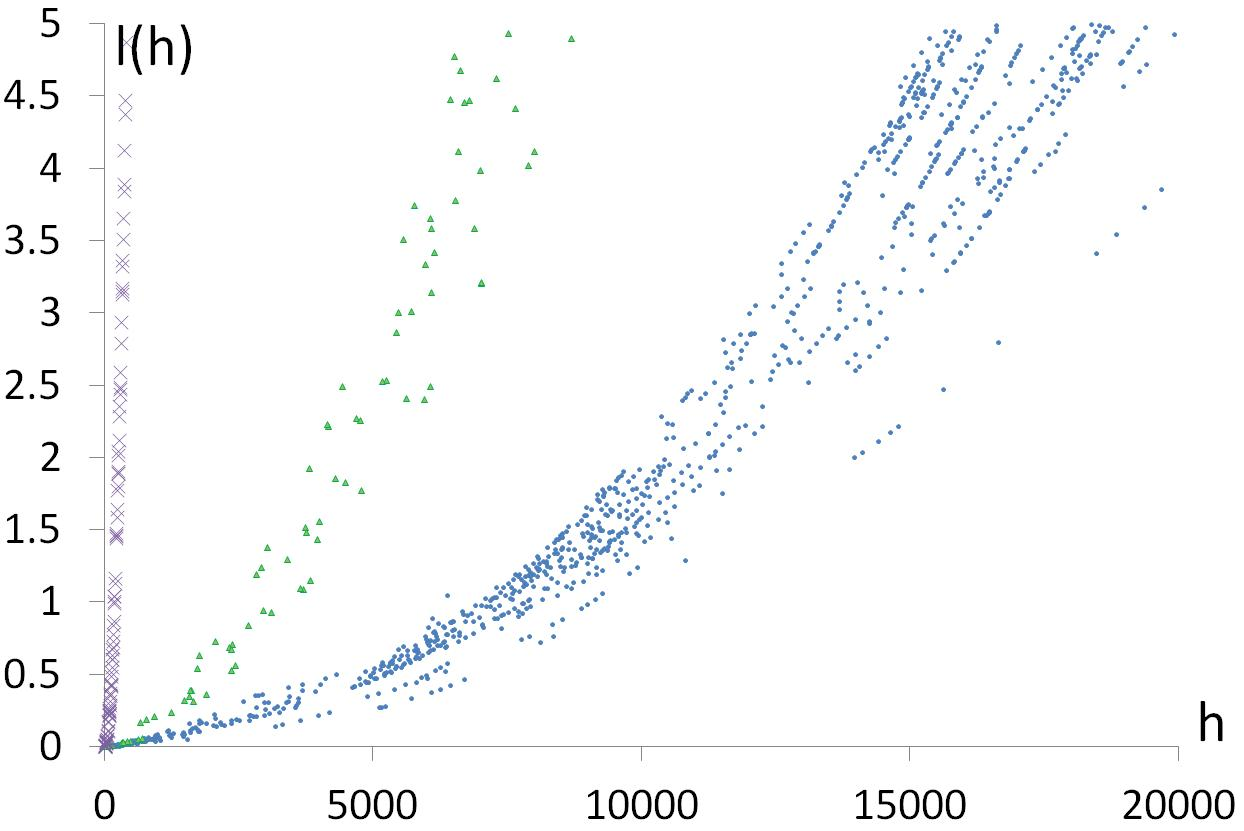
\includegraphics[width=0.77\linewidth]{Dyshaev-01}
	\caption{\footnotesize Функция $l(h)$ для различных инструментов}
	\label{fig:dyshaev-01}
\end{figure}

Для практического использования аппроксимацию $l$ степенной функцией $\varepsilon h^n$ необходимо проводить по левой границе множеств значений $l(h)$ с тем, чтобы при дельта"=хед\-жи\-ро\-ва\-нии учесть максимально возможную стоимость ликвидности. Наблюдения показывают, что вид функции $l(h)$ меняется в течение торгов, поэтому необходимо провести дальнейшие исследования для уточнения характера исследуемой зависимости, а именно для установления возможной зависимости  $n$ и $\varepsilon$ от  рыночных параметров.

% Оформление списка литературы
\smallskip \centerline {\bf Литература} \nopagebreak

1. {\it Rogers, L. C.~G., and Singh, S.} The cost of illiquidity and its effects on hedging. Mathematical Finance, vol.~20, no.~4, pp.~597--615.
